\chapter{Hash Table Implementation} % Write in your own chapter title
\label{Chapter3}
\lhead{Chapter 3. \emph{Hash Table Implementation}}


\begin{figure}[H]
	\centering
	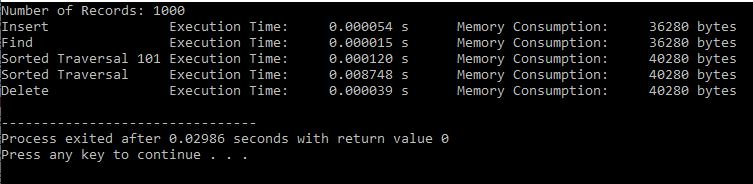
\includegraphics[scale =0.7]{./Figures/hash1000.jpg}
	\rule{35em}{0.5pt}
	\caption{Results for hash implementation with data size 1000.}
	\label{fig:Hash 1000}
\end{figure}

\begin{figure}[H]
	\centering
	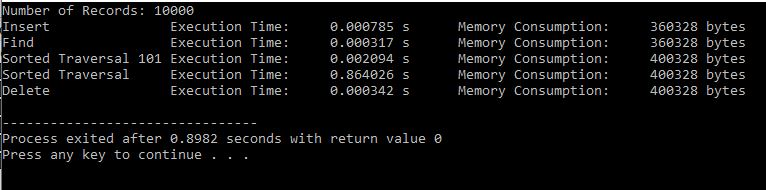
\includegraphics[scale =0.7]{./Figures/hash10000.jpg}
	\rule{35em}{0.5pt}
	\caption{Results for hash implementation with data size 10000.}
	\label{fig:Hash 10000}
\end{figure}

\begin{figure}[H]
	\centering
	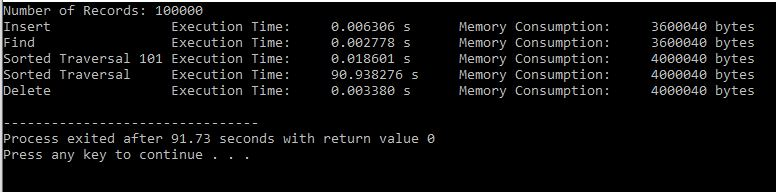
\includegraphics[scale =0.7]{./Figures/hash100000.jpg}
	\rule{35em}{0.5pt}
	\caption{Results for hash implementation with data size 100000.}
	\label{fig:Hash 100000}
\end{figure}

\begin{figure}[H]
	\centering
	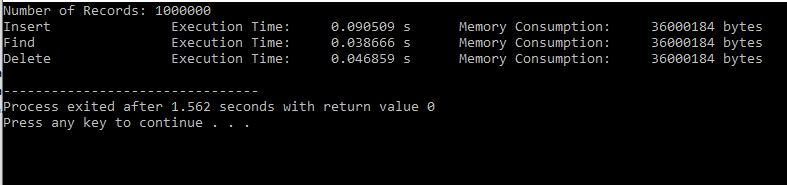
\includegraphics[scale =0.7]{./Figures/hash1000000.jpg}
	\rule{35em}{0.5pt}
	\caption{Results for hash implementation with data size 1000000.}
	\label{fig:Hash 1000000}
\end{figure}
